\documentclass[12pt,a4paper]{report}
\begin{comment}
\usepackage{amsmath,amsthm,amssymb,mathrsfs,graphicx}
\allowdisplaybreaks


\newtheorem{theorem}{Theorem}
\newtheorem{definition}{Definition}
\newtheorem{example}{Example}
\newtheorem{corollary}{Corollary}
\newtheorem{lemma}{Lemma}
\newtheorem{proposition}{Proposition}
\newtheorem{remark}{Remark}
\newtheorem{algorithm}{Algorithm}

\renewcommand{\baselinestretch}{1.5}
\end{comment}
\begin{document}

%DONE
%except to tack on last theorem?

\chapter{Groundwork}

In this chapter we will lay the groundwork necessary, and we will recall and state some necessary definitions and theorems. The two topics we will cover is Convex Geometry and Groebner bases.

All definitions and theorems are taken from \cite{AndersPHD} unless specified otherwise.

\section{Convex Geometry}
Here we will give some useful definitions and a couple of results. Several of these theorems, whilst not easy to prove, are relatively intuitive in nature and so we will merely state them. A standard reference for polyhedral and convex geometry can be found at \cite{StandardConvex}.

To begin, recall the definition of a fan in $\mathbb R^n$. 
A \emph{polyhedron} in $\mathbb R^n$ is defined to be a set of the form $\{x \in \mathbb R^n : Ax \leq b\}$, where $A \in \mathbb R^{n \times n}$ is a matrix, $b \in \mathbb R^{n}$ is a vector.
\begin{itemize}
\item Bounded polyhedra are called \emph{polytopes}.

\item If $b = 0$, the set $\{x \in \mathbb R^n : Ax \leq 0\}$ is called a \emph{polyhedral cone}.
\item The \emph{dimension}, or $dim(P)$, of a polyhedron P is the dimension of the smallest affine subspace containing it.

\item \emph{face} of a polyhedron P is a subset of P which is the set of maximizers of a linear form w over P, written in the following form:
\begin{equation*}
    face_{w} (P) := \{p \in P : \langle w,p \rangle = max_{q \in P} \langle w,q \rangle \}.
\end{equation*}

\item The face of a polyhedron is a polyhedron.
\item A face of P is called a \emph{facet} if its dimension is one smaller than the dimension of P.
\end{itemize}

\begin{definition}
A collection $C$ of polyhedra in $\mathbb R^n$ is called a \emph{polyhedral complex} if it has the following properties:
\begin{enumerate}
    \item all non-empty faces of a polyhedron $P \in C$ are in $C$.
    \item the intersection of any two polyhedra $A,B \in C$ is a face of A and a face of B.
\end{enumerate}
\end{definition}

\begin{itemize}
    \item The \emph{support}, or $supp(C)$ of C is the union of all the members of C. 
    \item A polyhedral complex is called a \emph{fan} if it only consists of cones. 
    \item One-dimensional cones of polyhedral fans are called rays.
    \item A polyhedral cone is said to be \emph{complete} if the support of a fan is $\mathbb R^n$.
    \item A polyhedral cone is \emph{pure} if all its maximal cones have the same dimension.
\end{itemize}

\begin{figure}
\begin{center}
    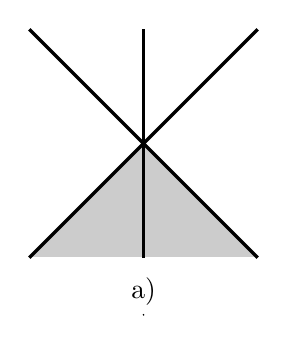
\begin{tikzpicture}[scale=0.725] %%First image
\draw[fill=black!20!white, draw=white] (0,0)--(-2,-2)--(0,-2)--(2,-2)--(0,0)--cycle;
\draw[very thick] (0,0) -- (0,2); %%Top
\draw[very thick] (0,0) -- (0,-2); %%Bottom
\draw[very thick] (0,0) -- (2,2); %%TopRight
\draw[very thick] (0,0) -- (-2,-2); %%BottomLeft
\draw[very thick] (0,0) -- (2,-2); %%BottomRight
\draw[very thick] (0,0) -- (-2,2); %%TopLeft
\filldraw[black] (0,-3) circle (0.1pt) node[anchor=south] {a)};
\end{tikzpicture}
\qquad
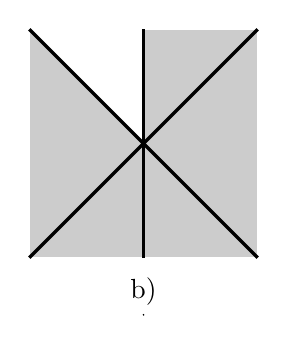
\begin{tikzpicture}[scale=0.725] %%Second image
\draw[fill=black!20!white, draw=white] (0,0)--(-2,2)--(-2,-2)--(0,-2)--(2,-2)--(2,2)--(0,2)--cycle;
\draw[very thick] (0,0) -- (0,2);
\draw[very thick] (0,0) -- (0,-2);
\draw[very thick] (0,0) -- (2,2);
\draw[very thick] (0,0) -- (-2,-2);
\draw[very thick] (0,0) -- (2,-2);
\draw[very thick] (0,0) -- (-2,2);
\filldraw[black] (0,-3) circle (0.1pt) node[anchor=south] {b)};
\end{tikzpicture}
\qquad
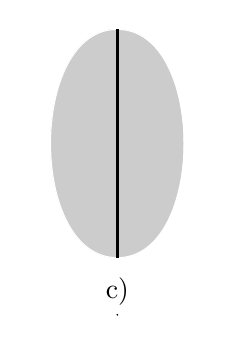
\begin{tikzpicture}[scale=0.725] %%Third image
\coordinate (A) at (0,-2);
\coordinate (B) at (0, 2);
\draw[fill=black!20!white, draw=white] (A) to [bend left=90] (B);
\draw[fill=black!20!white, draw=white] (A) to [bend right=90] (B);
\draw[very thick] (A)--(B);
\filldraw[black] (0,-3) circle (0.1pt) node[anchor=south] {c)};
\end{tikzpicture} 
\qquad
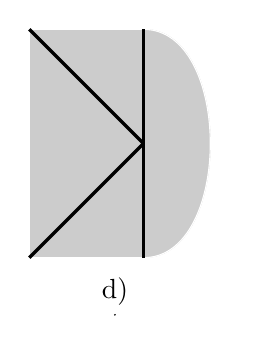
\begin{tikzpicture}[scale=0.725] %%Forth image
\coordinate (A) at (0,-2);
\coordinate (B) at (0, 2);
\draw[fill=black!20!white, draw=white] (A) to [bend right=90] (B);
\draw[fill=black!20!white, draw=white] (0,0)--(0,2)--(-2,2)--(-2,-2)--(0,-2)--cycle;
\draw[very thick] (A)--(B);
\draw[very thick] (0,0) -- (-2,2); %%TopLeft
\draw[very thick] (0,0) -- (-2,-2); %%BottomLeft
\filldraw[black] (-0.5,-3) circle (0.1pt) node[anchor=south] {d)};
\end{tikzpicture}
\end{center}
\caption{A collection of four different cones referenced in Example 2.1.2}
\end{figure}

\begin{example}
In Figure 2.1 there is a collection of different cones drawn. 
\begin{enumerate}[label=(\alph*)]
    \item This collection consists of: 1 zero-dimensional cone, 6 rays and 2 two-dimensional cones. This is a fan, however it is not complete (since the support of the fan is not $\mathbb{R}^{2}$), and it is not pure (since not all of its maximal cones have the same dimension).
    \item This collection consists of: 1 zero-dimensional cone, 6 rays and 5 two-dimensional cones. This is a fan and it is not complete (since the support of the fan is not $\mathbb{R}^{2}$), but it is pure (all maximal cones have same dimension).
    \item This collection of cones consists of: 1 line and 2 regions, both of which are half-spaces. This is a fan and it is both complete and pure.
    \item This collection of cones consists of: 1 zero-dimensional, 4 rays, 1 line and 4 regions, one of which is a half-space. The existence of this half-space means that this is not a polyhedral fan, due to the fact that intersections of other regions with this half-space is not a face of the same half-space.
\end{enumerate}
\end{example}

An important fact to notice is that, for a finite non-empty fan, the intersection of all cones is a subspace. This subspace is the smallest non-empty face of every cone in the fan.

A simple way to construct a fan is taking the $\emph{normal fan}$ of a polyhedron.

\begin{definition}
Let $P \subseteq \mathbb R^{n}$ be a polyhedron. For a face F of P we define its \emph{normal cone}:
\begin{equation*}
    N_{P} (F):= \overline{ \{ w \in \mathbb{R}^{n} : face_{w} (P) = F \} }
\end{equation*}
with the closure being taken in the Euclidean topology. 

The \emph{normal fan} of P is the fan consisting of the normal cones $N_P (F)$ as F runs through all non-empty faces of P.
\end{definition}

The following equation is satisfied for a non-empty face F:
\begin{equation*}
    dim(N_{P} (F)) + dim(F) = n.
\end{equation*}

Using this, we can see that the support of the normal fan of a polytope is $\mathbb R^n$, or as defined before, complete.

\begin{definition}
The \emph{common refinement} of two fans $F_{1}$ and $F_{2}$ in $\mathbb R^{n}$ is defined as
\begin{equation*}
    F_{1} \wedge F_{2} = \{C_{1} \cap C_{2} \}_{(C_{1},C_{2}) \in F_{1} \times F_{2}}
\end{equation*}


The \emph{common refinement} of two fans is also a fan.
\end{definition}

\begin{definition}
The \emph{Minkowski sum} of two polyhedra $P,Q \subseteq \mathbb R^{n}$ is the polyhedron:
\begin{equation*}
    P + Q := \{p + q: (p,q) \in P \times Q \}
\end{equation*}
\end{definition}

\begin{proposition}
Let $P,Q \subseteq \mathbb R^{n}$ be two polyhedra. The normal fan of $P + Q$ is the common refinement of the normal fan of P and the normal fan of Q.
\end{proposition}

\begin{definition}
The \emph{relative interior} of a polyhedron $P \subseteq \mathbb R^{n}$ is the interior of $P \cap L \subseteq L$ where L is the smallest affine subspace of $\mathbb R^{n}$ containing P. Here L has its topology induced from the Euclidean topolgy of $\mathbb R^{n}$.
\end{definition}

We denote the relative interior by $Rel Int(P)$.

Why would use relative interior over interior? We will briefly explore this using a simple example. Firstly, note that relative interior is a refinement of the concept of interior, and it is useful for dealing with lower-dimensional sets in higher-dimensional spaces. An example of this is the set of points $(x, y, 0)$ restricted by $x^2 + y^2 \leq 1$ in $\mathbb{R}^{3}$. If we take the interior of this set, we find that the interior is in fact empty. Why? It is due to how interior is defined i.e. a point $p$ is said to be in the interior if we can construct an open ball around $p$, and the open ball is itself contained within the set (in this $x^2 + y^2 \leq 1$). Any open ball drawn around $p = (x, y, 0)$ will involve points that do not lie on the $xy$-plane, and hence no points cannot be in the interior, and so it is empty.

While this is perfectly correct, it is not really useful and fails to capture any information. By using relative interior, we instead look at the affine subspace, which is $\mathbb{R}^{2}$ (not $\mathbb{R}^{3}$), and so we construct open balls only in the $xy$-plane and ignore the $z$ dimension. This means that the relative interior is, instead of being empty, the interior of the unit disc, as we would expect.  

\begin{definition}
For a polynomial $f$ we can define:
\begin{equation*}
    \partial_{<} (f) = \{ u - u^{'} \mid u^{'} \in \text{supp}(f) \setminus \{u \} \} \in \mathbb Z^{n}
\end{equation*}
and for a set of polynomials $F$ we can define:
\begin{equation*}
    \partial_{<} (F) = \cup_{f \in F} \partial_{<} (f)
\end{equation*}
\end{definition}

\section{Groebner Bases}
We will not go over the very basics of Groebner basis theory (see: division algorithm for multivariate polynomials, Buchberger's Algorithm, S-polynomials), and if needed \cite{StandardGroebner} can be used as a reference. This chapter will serve as a quick refresher to both outline the notation used as well as some important information about marked Groebner bases and homogeneous ideals. 

Let $R = K[x_{1}, \ldots, x_{n}]$ be a polynomial ring over a field $K$, with $n$ different variables and let $I \subseteq R$ be an ideal. For $\alpha \in \mathbb N^{n}$ we use the notation $x^{\alpha} := x_{1} ^{\alpha_{1}} \ldots x_{n} ^{\alpha_{n}}$ to denote a monomial in R. 

By a \emph{term ordering} (or monomial ordering) on R we mean a total ordering  $<$ on all monomials in R such that:

\begin{enumerate}
    \item For all $\alpha \in \mathbb {N}^{n} \setminus \{0\} : 1 < L x^{\alpha}$ and
    \item for all $\alpha, \beta, \gamma \in \mathbb N^{n} : x^{\alpha} < x^{\beta} \Rightarrow x^{\alpha} x^{\gamma} < x^{\beta} x^{\gamma}$
\end{enumerate}


A total ordering is a binary relation (here it is $<$), that has the properties of antisymmetry, transitivity and convexity. By term we mean a monomial together with its associated coefficient. We use term orders for ordering terms, ignoring their coefficients. 

Note: We are using $<$ for our total ordering notation instead of the more standard notation of $\prec$. We do this in view of reserving this notation for the new ordering (a preordering) we will be introducing later and making it easier to distinguish between the two types of orderings.


For a vector $w \in \mathbb{R}_{n} ^ {\geq 0}$ and a term order $<$ we define a new term order $<_{w}$ as follows:
\begin{equation*}
    x^{\alpha} <_{w} x^{\beta} \Leftrightarrow \langle w, \alpha \rangle < \langle w, \beta \rangle \vee (\langle w, \alpha \rangle = \langle w, \beta \rangle \wedge x^{\alpha} < x^{\beta})
\end{equation*}

Let $<$ be a term order. For a non-zero polynomial $f \in R$ we define its \emph{initial term}, $\initial_{<} (f)$, to be the unique maximal term of f with respect to our term order $<$. In the same way for $w \in \mathbb R^{n}$ we define the \emph{initial form}, $\initial_{w} (f)$, to be the sum of all terms of $f \in R$ whose exponents maximize $\langle w, \cdot \rangle$. For a non-zero polynomial f we have the following: $\initial_{{<}_{w}} (f) = \initial_{<} (\initial_{w} (f))$. We define the \emph{Newton polytope} of a polynomial $f$ to be the convex hull of its exponent vectors.

\begin{remark}
Let $f \in K[x_{1}, \ldots ,x_{n}]$ be a polynomial and $P \subseteq \mathbb R^{n}$ its Newton polytope. Notice that $\initial_{u} (f) = \initial_{v} (f) \Leftrightarrow face_{u} (P) = face_{v} (P)$ and that $\initial_{u} (f)$ is a monomial if and only if $face_{u} (P)$ has dimension 0 or, equivalently, the normal cone $N_{P} (face_{u} (P))$ is full-dimensional.
\end{remark}

The \emph{w-degree} of a term $cx^{\alpha}$ is $\langle w, \alpha \rangle$ and the \emph{w-degree} of a non-zero polynomial f is the \emph{w-degree} of the terms of $\initial_{w} (f)$. The \emph{initial ideal} of an ideal I with respect to both $<$ and $w$ are defined as:


$\initial_{<} (I) = \langle \initial_{<} (f): f \in I \setminus \{0 \} \rangle$ and $\initial_{w} (I) = \langle \initial_{w} (f): f \in I \rangle$.

It is important to point out that $\initial_{<} (I)$ is a monomial ideal, however $\initial_{w} (I)$ may not be a monomial ideal. A monomial in $R \setminus \initial_{<} (I)$ (with coefficient 1) is called a \emph{standard monomial} of $\initial_{<} (I)$. Although initial ideals are defined with respect to vectors that may negative, we note that Groebner bases are only defined with respect to true term orders:

\begin{definition}
Let $I \subseteq R$ be an ideal and $<$ a term order on R. A generating set $G = \{g_{1}, \ldots ,g_{m} \}$ for I is called a \emph{Groebner basis} for I with respect to $<$ if: 
\begin{equation*}
    \initial_{<} (I) = \langle \initial_{<} (g_{1}, \ldots , \initial_{<} (g_{m}) \rangle.
\end{equation*}
\end{definition}

The Groebner basis $G$ is \emph{minimal} if $\{ \initial_{<} (g_{1}, \ldots , \initial_{<} (g_{m}) \}$ generates $\initial_{<} (I)$ minimally.
A minimal Groebner basis is said to be \emph{reduced} if the initial term of every $g \in G$ has coefficient 1 and all other monomials in g are standard monomials of $in_{<} (I)$.


We use  \emph{marked} Groebner basis for a Groebner basis where the initial terms are marked, to clearly differentiate them from any other non-initial terms. As a simple example, $\{ \underline{x^3} + xyz + y^3 + z^3 \}$, $\{ x^3 + xyz + \underline{y^3} + z^3 \}$ and $\{ x^3 + xyz + y^3 + \underline{z^3} \}$ are marked Groebner basis for the ideal $\langle x^3 + xyz + y^3 + z^3 \rangle$, however $\{ x^3 + \underline{xyz} + y^3 + z^3 \}$ is not, due to the fact that $xyz$ cannot be the leading term under any given term order.

Given a marking of one term of each polynomial in a set $G \subseteq R$, the division algorithm produces the remainder of a polynomial $f \in R$ modulo $G$. Due to how Buchberger's Algorithm functions, the remainder output from the algorithm depends on the order in which these reduction steps are applies. If $G$ is a marked Groebner basis with respect to a term order $<$, then the remainder is uniquely determined, and we denote it as the \emph{normal form} of f modulo G. This so-called normal form is only dependent on the term markings on the Groebner basis and the term order.

For a term order $<$ and an ideal I, Buchberger's algorithm guarantees the existence of a unique marked reduced Groebner basis. We denote this by $G_{<} (I)$. Buchberger's algorithm is a completion procedure that keeps adding remainders of S-polynomials to a generating set of I until Buchberger's S-criterion is satifsfied:

\begin{theorem}
Let $I \subseteq R$ be an ideal and $<$ a term order. A polynomial set $G \subseteq R$ marked according to $<$ is a Groebner basis of I with respect to $<$ if for all $g_{1}, g_{2} \in G$ some remainder of the division algorithm run on $S(g_{1}, g_{2})$ modulo G is zero. 
\end{theorem}
Here $S(g_{1}, g_{2})$ is the \emph{S-polynomial} $c_{2} x^{({v_{1} \vee v_{2})} - v_{1}} g_{1} - c_{1} x^{({v_{1} \vee v_{2})} - v_{2}} g_{2}$, assuming that $c_{i} x^{v_{i}}$ is the marked term of $g_{i}$ with $c_{i} \in k$ and $v_{i} \in \mathbb N^{n}$ for $i = 1, 2$ and with $v_{1} \vee v_{2}$ being the coordinate-wise maximum of $v_{1}$ and $v_{2}$



\begin{remark}
For two term orders $<$ and $<^{'}$, if $\initial_{<} (I) = \initial_{{<}^{'}} (I)$ then $G_{<} (I) = G_{{<}^{'}} (I)$. To show that this is the case, take a polynomial $g \in G_{<} (I)$. We know that $G_{<} (I)$ is reduced, so only the marked term of g is in $\initial_{<} (I)$. Hence we can say $\initial_{{<}^{'}} (g)$, which is in $\initial_{{<}^{'}} (I) = \initial_{<} (I)$ must be the same marked term. This shows, no matter what term order we consider, the S-polynomials of elements in $G_{<} (I)$ are the same. Hence, all S-polynomials have remainder zero. This proves that $G_{<} (I)$ is also a Groebner basis with respect to $<^{'}$ as well as $<$. Since it is also reduced, we can use uniqueness of reduced Groebner bases and show that $G_{<} (I) = G_{{<}^{'}} (I)$.

Conversely, given some marked Groebner basis $G_{<} (I)$, the initial ideal $\initial_{<} (I)$ can easily be found.
\end{remark}

Let $w \in \mathbb R^{n}$. A polynomial $f \in R$ is \emph{w-homogeneous} if $\initial_{w} (f) = f$. An ideal $I \subseteq R$ if it is generated by w-homogeneous elements. Hilbert's basis theorem states that $I$ has a finite generating set. Each generator in the set can be expressed in term of finitely many w-homogeneous generators. This proves that $I$ has a finite generating set consisting of w-homogeneous elements. Using the w-homogeneous generating set, a polynomial $f \in I$ can be uniquely written sum $f = \sum_{i} f_{i}$ where the $f_{i}$'s are w-homogeneous, have different w-degrees and belong to $I$. Using this we can deduce the following lemmas.

\begin{lemma}
Let $I \subseteq R$ be an ideal and $w \in \mathbb R^{n}$. Then I is w-homogeneous if and only if $\initial_{w} (I) = I$.
\end{lemma}

\begin{lemma}
Let $I \subseteq R$ be an w-homogenous ideal with $w \in \mathbb R^{n}$ and $v \in \mathbb R^{n}$. Then $\initial_{v+sw} (I) = \initial_{v} (I)$ for any $s \in \mathbb R$.

We say that an ideal is homogeneous if it is w-homogeneous for $w = (1, \cdots, 1)$.
\end{lemma}

Notice that if Buchberger's algorithm gets w-homogeneous generators as input, then the output is also w-homogeneous. In particular, all reduced Groebner bases for an w-homogeneous ideal consists of w-homogeneous elements. As a consequence equations defining the subspace of vectors for which I is homogeneous can be read off from any reduced Groebner basis. We conclude that $G_{>} (I) = G_{{>}_{w}} (I)$ for any term order if I is w-homogeneous with $w \in \mathbb R_{\geq 0}^{n}$.

\begin{remark}
We may be less strict with our ordering if we are given homogeneous generators for an ideal. Let $>$ be an ordering which is a term order except that it does not satisfy $1 < x^{\alpha}$ for $\alpha \in \mathbb N^{n} \setminus {0}$. Then $<$ has the property that it will give the same reduced Groebner basis as $<_{w}$ when run on an w-homogeneous generating set. One example of this is the reverse lex ordering which only makes sense for homogeneous generating sets (with respect to a positive grading w). For $x_{n} < x_{n-1} < \ldots < x_{1}$ it is defined as follows:
\begin{equation*}
    x^{u} < x^{v} \Leftrightarrow \exists j: u_{j} > v_{j} \wedge \forall i > j: u_{i} = v_{i}
\end{equation*}
\end{remark}

\begin{definition}
Let $A \in GL_{n} (\mathbb R)$ be an invertible matrix. If the first non-zero entry in each column is positive then the matrix defines a matrix term order $<_{A}$ in the following way. We define $x^{\alpha} <_{A} x^{\beta}$ whenever the first non-zero entry $A(a-b)$ is negative, where $a, b \in \mathbb N^{n}$.
\end{definition}

\begin{lemma}
Let $A \in \mathbb R^{n \times n}$ be a matrix defining a term order and let $a, b \in \mathbb N^{n}$. We define $A_{\epsilon} = \epsilon ^{0} A_{1} + \epsilon ^{1} A_{2} + \ldots + \epsilon ^{n-1} A_{n}$ where $A_{i}$ is the i-th row of A. For all $\epsilon > 0$ sufficiently small we have $x^{\alpha} <_{A} x^{\beta}$ if and only if $A_{\epsilon} \cdot a < A_{\epsilon} \cdot b$.
\end{lemma}

\begin{proof}
Assume that $a \neq b$, and let $M \in \mathbb R_{>0}$ be a number, which is numerically larger than any value in $A(a-b)$. Also let L be the first non-zero entry of $A(a-b)$. For every positive $\epsilon < \frac{|L|}{nM}$, we can show that the sign of $A_{\epsilon} (a-b)$ is the same sign of $L$.

In the case that $L > 0$, then, we have $\epsilon > 0$. Since $nM > |L|$, we can also say that $\epsilon < 1$. Hence we can approximate $A_{\epsilon} (a-b)$ by the first non-zero term, $\epsilon^{n-1} A_{n}$, or $\epsilon^{n-1} L$. Since both $\epsilon^{n-1}$ and $L$ are positive, then we can say $A_{\epsilon} (a-b)$ is also positive, the same sign as $L$.

In the case that $L < 0$, we can make the same arguments except that $\epsilon^{n-1} L$ is now negative, the same sign as $L$.
\end{proof}

An important result concerning term orders is the following theorem which states that any term order has a matrix representation.

\begin{theorem}\cite{LRobbiano}
Let $<$ be a term order on $k[x_{1}, \ldots ,x_{n}]$. There exists a matrix $T \in \mathbb R^{n \times n}$ with rows $\tau_{1}, \ldots ,\tau_{n}$ such that for $u, v \in \mathbb N^{n}$:

$x^{u} < x^{v} \Leftrightarrow \exists j: \langle \tau_{j}, u \rangle < \langle \tau_{j}, v \rangle \wedge \forall i < j: \langle \tau_{i}, u \rangle = \langle \tau_{i}, v \rangle$
\end{theorem}

\end{document}